

\tikzset{every picture/.style={line width=0.75pt}} %set default line width to 0.75pt        

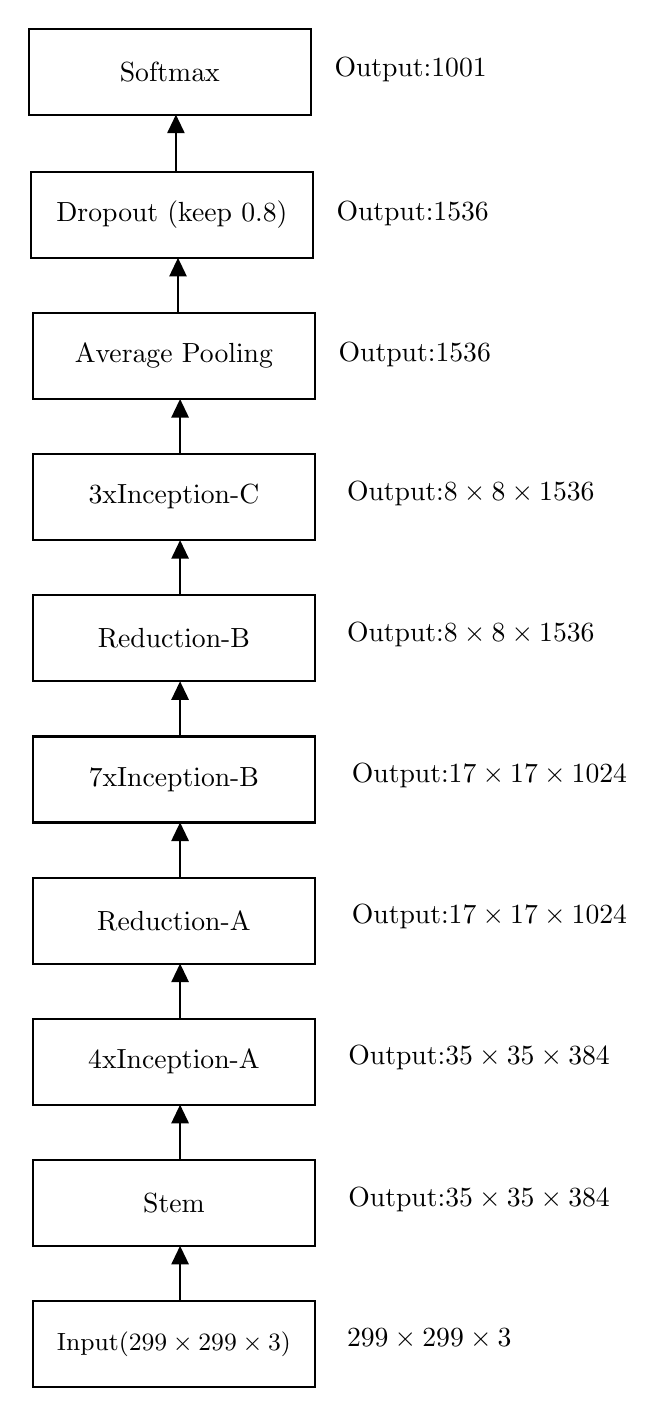
\begin{tikzpicture}[x=0.75pt,y=0.75pt,yscale=-1,xscale=1]
%uncomment if require: \path (0,742.7142868041992); %set diagram left start at 0, and has height of 742.7142868041992

%Flowchart: Process [id:dp9253173394290999] 
\draw   (98,621) -- (233.93,621) -- (233.93,662.43) -- (98,662.43) -- cycle ;
%Flowchart: Process [id:dp47578347996398307] 
\draw   (98,553) -- (233.93,553) -- (233.93,594.43) -- (98,594.43) -- cycle ;
%Straight Lines [id:da2925025767777827] 
\draw    (168.93,621.43) -- (168.93,596.43) ;
\draw [shift={(168.93,594.43)}, rotate = 450] [fill={rgb, 255:red, 0; green, 0; blue, 0 }  ][line width=0.75]  [draw opacity=0] (8.93,-4.29) -- (0,0) -- (8.93,4.29) -- cycle    ;

%Flowchart: Process [id:dp5382364848384393] 
\draw   (98,485) -- (233.93,485) -- (233.93,526.43) -- (98,526.43) -- cycle ;
%Straight Lines [id:da06940381159807729] 
\draw    (168.93,553.43) -- (168.93,528.43) ;
\draw [shift={(168.93,526.43)}, rotate = 450] [fill={rgb, 255:red, 0; green, 0; blue, 0 }  ][line width=0.75]  [draw opacity=0] (8.93,-4.29) -- (0,0) -- (8.93,4.29) -- cycle    ;

%Flowchart: Process [id:dp21301144435418706] 
\draw   (98,417) -- (233.93,417) -- (233.93,458.43) -- (98,458.43) -- cycle ;
%Straight Lines [id:da45627711718103714] 
\draw    (168.93,485.43) -- (168.93,460.43) ;
\draw [shift={(168.93,458.43)}, rotate = 450] [fill={rgb, 255:red, 0; green, 0; blue, 0 }  ][line width=0.75]  [draw opacity=0] (8.93,-4.29) -- (0,0) -- (8.93,4.29) -- cycle    ;

%Flowchart: Process [id:dp7231968775803179] 
\draw   (98,349) -- (233.93,349) -- (233.93,390.43) -- (98,390.43) -- cycle ;
%Straight Lines [id:da7165121439179447] 
\draw    (168.93,417.43) -- (168.93,392.43) ;
\draw [shift={(168.93,390.43)}, rotate = 450] [fill={rgb, 255:red, 0; green, 0; blue, 0 }  ][line width=0.75]  [draw opacity=0] (8.93,-4.29) -- (0,0) -- (8.93,4.29) -- cycle    ;

%Flowchart: Process [id:dp20620702942862734] 
\draw   (98,281) -- (233.93,281) -- (233.93,322.43) -- (98,322.43) -- cycle ;
%Straight Lines [id:da10564528480224444] 
\draw    (168.93,349.43) -- (168.93,324.43) ;
\draw [shift={(168.93,322.43)}, rotate = 450] [fill={rgb, 255:red, 0; green, 0; blue, 0 }  ][line width=0.75]  [draw opacity=0] (8.93,-4.29) -- (0,0) -- (8.93,4.29) -- cycle    ;

%Flowchart: Process [id:dp6409642010028676] 
\draw   (98,213) -- (233.93,213) -- (233.93,254.43) -- (98,254.43) -- cycle ;
%Straight Lines [id:da583110185704452] 
\draw    (168.93,281.43) -- (168.93,256.43) ;
\draw [shift={(168.93,254.43)}, rotate = 450] [fill={rgb, 255:red, 0; green, 0; blue, 0 }  ][line width=0.75]  [draw opacity=0] (8.93,-4.29) -- (0,0) -- (8.93,4.29) -- cycle    ;

%Flowchart: Process [id:dp747253235525678] 
\draw   (98,145) -- (233.93,145) -- (233.93,186.43) -- (98,186.43) -- cycle ;
%Straight Lines [id:da9482962038382927] 
\draw    (168.93,213.43) -- (168.93,188.43) ;
\draw [shift={(168.93,186.43)}, rotate = 450] [fill={rgb, 255:red, 0; green, 0; blue, 0 }  ][line width=0.75]  [draw opacity=0] (8.93,-4.29) -- (0,0) -- (8.93,4.29) -- cycle    ;

%Flowchart: Process [id:dp47103409298757426] 
\draw   (97,77) -- (232.93,77) -- (232.93,118.43) -- (97,118.43) -- cycle ;
%Straight Lines [id:da30249651940608824] 
\draw    (167.93,145.43) -- (167.93,120.43) ;
\draw [shift={(167.93,118.43)}, rotate = 450] [fill={rgb, 255:red, 0; green, 0; blue, 0 }  ][line width=0.75]  [draw opacity=0] (8.93,-4.29) -- (0,0) -- (8.93,4.29) -- cycle    ;

%Flowchart: Process [id:dp5661311837160838] 
\draw   (96,8) -- (231.93,8) -- (231.93,49.43) -- (96,49.43) -- cycle ;
%Straight Lines [id:da5142446239913938] 
\draw    (166.93,76.43) -- (166.93,51.43) ;
\draw [shift={(166.93,49.43)}, rotate = 450] [fill={rgb, 255:red, 0; green, 0; blue, 0 }  ][line width=0.75]  [draw opacity=0] (8.93,-4.29) -- (0,0) -- (8.93,4.29) -- cycle    ;


% Text Node
\draw (165.96,641.71) node  [align=left] {{\small Input($\displaystyle 299\times 299\times 3$)}};
% Text Node
\draw (165.96,573.71) node  [align=left] {Stem};
% Text Node
\draw (289,639) node  [align=left] {$\displaystyle 299\times 299\times 3$};
% Text Node
\draw (313,572) node  [align=left] {Output:$\displaystyle 35\times 35\times 384$};
% Text Node
\draw (165.96,505.71) node  [align=left] {4xInception-A};
% Text Node
\draw (313,504) node  [align=left] {Output:$\displaystyle 35\times 35\times 384$};
% Text Node
\draw (165.96,437.71) node  [align=left] {Reduction-A};
% Text Node
\draw (318,436) node  [align=left] {Output:$\displaystyle 17\times 17\times 1024$};
% Text Node
\draw (165.96,369.71) node  [align=left] {7xInception-B};
% Text Node
\draw (318,368) node  [align=left] {Output:$\displaystyle 17\times 17\times 1024$};
% Text Node
\draw (165.96,301.71) node  [align=left] {Reduction-B};
% Text Node
\draw (309,300) node  [align=left] {Output:$\displaystyle 8\times 8\times 1536$};
% Text Node
\draw (165.96,233.71) node  [align=left] {3xInception-C};
% Text Node
\draw (309,232) node  [align=left] {Output:$\displaystyle 8\times 8\times 1536$};
% Text Node
\draw (165.96,165.71) node  [align=left] {Average Pooling};
% Text Node
\draw (282,165) node  [align=left] {Output:$\displaystyle 1536$};
% Text Node
\draw (164.96,97.71) node  [align=left] {Dropout (keep $\displaystyle 0.8$)};
% Text Node
\draw (281,97) node  [align=left] {Output:$\displaystyle 1536$};
% Text Node
\draw (163.96,28.71) node  [align=left] {Softmax};
% Text Node
\draw (280,28) node  [align=left] {Output:$\displaystyle 1001$};


\end{tikzpicture}